\documentclass[paper=a4, fontsize=11pt]{article}

\usepackage[utf8]{inputenc}
\usepackage[english]{babel}
\usepackage{sectsty}
\usepackage{listings}
\usepackage{graphicx}
\usepackage{wrapfig}
\usepackage[backend=biber,style=authoryear-icomp]{biblatex}
\usepackage{caption,subcaption}
\usepackage{datetime}

\newdate{date1}{11}{11}{2019}
\newdate{date2}{16}{12}{2019}
\newdate{missed}{15}{11}{2019}
\newdate{late}{16}{12}{2019}

\usepackage{fancyhdr}

\usepackage{blindtext}
\renewcommand{\subsectionmark}[1]{\markright{\thesubsection\ #1}}

\pagestyle{fancy}
\fancyhf{}
\fancyfoot[C]{\thepage}
\fancyhead[C]{I Know You!}
\fancyhead[R]{Nicolà Lohr}
\fancyhead[L]{\nouppercase{\leftmark}}
\fancyheadoffset[R,L]{0cm}
\renewcommand{\headrulewidth}{0.5pt}


\usepackage{calc}
\setlength\textwidth{7in}
\setlength\textheight{9.5in}
\setlength\oddsidemargin{(\paperwidth-\textwidth)/2 - 1in}
\setlength\topmargin{(\paperheight-\textheight-\headheight-\headsep-\footskip)/2 - 1in}




%stickynote
\usepackage{xparse}
\usepackage{tikz}
\usetikzlibrary{shadows}
\usepackage{lipsum}

\definecolor{myyellow}{RGB}{242,226,149}

\NewDocumentCommand\StickyNote{O{7cm}mO{10cm}}{%
\begin{tikzpicture}
\node[
drop shadow={
shadow xshift=2pt,
shadow yshift=-4pt
},
inner xsep=7pt,
fill=myyellow,
xslant=-0.1,
yslant=0.1,
inner ysep=10pt
] {\parbox[t][#1][c]{#3}{#2}};
\end{tikzpicture}%
}


\allsectionsfont{\centering \normalfont\scshape}
\linespread{1.5}
\setlength{\parindent}{0pt}
\setlength{\parskip}{8pt}

\addbibresource{sources.bib}
\defbibheading{online}{\subsection{Online-Quellen}}
\defbibheading{offline}{\subsection{Literatur}}


\title{\normalfont \normalsize \textsc{KSZ, Kantonsschule Zug} \\ [25pt]
\huge I Know You!\linebreak\linebreak \large Metadata Analysis\\
}
\author{Nicolà Lohr\\[0.5cm]{\small Supervisor: Marco Schmid}}

\date{\normalsize\today}

\begin{document}


\clearpage
\newcommand{\HRule}{\rule{\linewidth}{0.5mm}}

\begin{center}


%\includegraphics[width=0.5\linewidth]{./kks.jpg}
\textsc{\Large  KSZ, Kantonsschule Zug}\\[0.8cm]

\vfill

% Title
\HRule \\[1.8cm]
\textsc{\Large  Wi-Fi metadata analysis}\\[0.8cm]
\textsc{ \huge  I Know You!}\\[1.4cm]

\HRule \\[1.5cm]

% Author and supervisor
\begin{minipage}[t]{0.38\textwidth}
\begin{flushleft} \large
\emph{Author:}\\
Nicolà Lohr \\ 


\end{flushleft}
\end{minipage}
\begin{minipage}[t]{0.6\textwidth}
\begin{flushright} \large
\emph{Supervisor:}\\
Marco Schmid
\end{flushright}
\end{minipage}

\vfill

% Bottom of the page
{\large \today}

\end{center}
\thispagestyle{empty}
\newpage
\thispagestyle{empty}
\newpage
\linespread{1}
\tableofcontents
\linespread{1.5}
\newpage
\begin{abstract}
%third person
In my project, I used passively collected Wi-Fi metadata to identify the user behind the MAC address. I was able to identify 80\% of the users. This includes their class, place of residence, first year at school, name, and best friends.
Intending to distribute the knowledge of the dangers of Big Data, I hung up posters and created a website to inform students at my school.

I looked shortly into the legal framework of Switzerland, the EU, and the USA. Compared to the CH and the EU, US citizens have quite a different opinion on data protection; comfort is preferred over privacy.

Alternative tracking methods were evaluated like RFID, Bluetooth, cameras, and how these are used in daily life.

The only defense against Big Data is to make it as hard as possible. This is possible with random or anonymous usernames, scramble all patterns, and minimize the amount of data produced by turning off or disabling Wi-Fi, Bluetooth and cellular when not needed.
\end{abstract}

\section{Introduction}
Big Data is a powerful tool that is used by many companies and governments to profile customers and citizens.

I wanted to create my own Big Data project to show how much information I can collect with seemingly harmless data and how easy this is. Imagine this omnipresent data like a cloud hanging over each person, created by today's technology. Every minute phones, laptops, headphones, and many electronic devices produce enormous amounts of data, yet mostly unnoticed by their users. In my project, I was just watching these clouds. I was a passive collector of this data, undetectable and unseen.

Many companies are using Big Data algorithms to improve sales and profit. A supermarket can track a person through the whole store.
Most people carries a mobile phone or a simple contactless credit or debit card, which can be tracked. The store knows exactly where a person walks through and in which alley they spend the most time in\footcite{supermarkettracking}. This is much simpler than using monitoring cameras where data extraction and evaluation are complex and expensive. In the end, when customers buy their products with a credit card, the supermarket also knows what they acquired. With this knowledge at hand, they start reordering the shelves, trying to make you purchase high-profit items or higher quantities. With a bonus card, the customer even voluntary provides more information, including his name and home address. Humankind is too greedy and ignorant to keep its data, even when it receives only 1\% of the bought value back to the bonus card.\footcite{supermarketpoints} A modern supermarket can figure out ones salary, age, gender, marital status, and much more by only looking at a users path and the items obtained at the end. \footcite{supermarketbigdata}

Some companies, for example, "GoogleAds," profile users online. They track which websites users visited and how long they stayed there. \footcite{googleadshow} As in the store, this data is used to increase profit by luring people into buying more. This time it is managed by showing you ads that have the most influence on you. 

Considering that a person repeatedly visits websites about sights and hotels for a London holiday trip, but never actually books it. Showing a targeted advertisement, offering a \emph{special} discount, with \emph{only a few left!} might close the deal. Profit made!

I had no access to a credit card tracker nor the information on who visited which site. But I was able to obtain access to the Wi-Fi-metadata. Wi-Fi-metadata is the information sent unencrypted over the air. They contain a minimum of personal information. Only with a small part of the data cloud, I could still get enough information to identify the owner of each device. In my thesis, I used MAC-addresses to differentiate each device. The MAC-address is a factory-set unique ID of the machine. This process makes the MAC difficult ot change and, therefore, distinguishable. This address is sent every time the device uses the Wi-Fi. With this information only, I tried to find out as much as possible about the students at my school. I was surprised by how much I found out.

\section{Approach}
The WiFi Pineapple is a small computer built to collect the data from the air efficiently.\footcite{wifipineapple}
I placed the WiFi Pineapple at the main entrance of my school. Most of the students walk by this point when entering and leaving the school. Their devices spread an enormous amount of data into the air. This data is the foundation of my analysis.

\begin{figure}[ht]
\centering
\begin{subfigure}[b]{0.45\linewidth}
\centering\includegraphics[width = 0.9\linewidth]{images/WIFIpineappleinside2.jpg}
\caption{\label{fig:WIFI-pineapple}}
\end{subfigure}
\begin{subfigure}[b]{0.45\linewidth}
\rotatebox[origin=c]{0}{\includegraphics[width = 0.9\linewidth]{images/WIFIpineappleinside1.jpg}}
\centering\caption{\label{fig:Hidden-WIFI-pineapple}}
\end{subfigure}
\caption{(\subref{fig:WIFI-pineapple}) shows the WiFi Pineapple and (\subref{fig:Hidden-WIFI-pineapple}) shows the placement of the WiFi Pineapple.}
\end{figure}

I know now when a specific device passed the WiFi Pineapple. The school publishes all the current time tables of all classes on its website.\footcite{stundenplan}
Linking the collected data with the time-table is straight forward. I looked only at the arrival time and the leaving time of the students to simplify my data. I assumed that a student leaves school as soon as he was allowed to and returns the next morning only shortly before his lessons started. I expected students to arrive at about ten to twenty minutes before their courses start. Then I compare each student to every class. I demonstrate this with the class 3H. Depending on how close the values of the students are to the ones I expect for the 3H, I give the class points. The more points the class has, the likelier it is that this student is in 3H. I give points relative to how close the student was to this time-span. With only one morning, the class 3H, 5B, 2F, and a few others would all have the same value because all of these classes start at the same time. But expanding the data to a week, 3H has a unique pattern. Therefore all members of the class 3H receive the best correlation. Different mornings have different importance. For example, if someone arrives on a Wednesday morning in time for the earliest lesson, there are still 51 possible classes for this student. But if he comes on time for the third lesson, there are only two potential classes he could be in. This importance level is explainable through the extra classes or the fact that the first two grades have off on Wednesday afternoon. 

Another interesting information I could work out was who is friends with whom. I assumed that friends are people walking together when school is over.

There are two reasons why I only look at afternoons to match friends. First reason: Arrival times depend mainly on the place of residence. Second reason: Most friends gather at school socialize when school begins, during lunch or after school.
Everyone who walks by my listening device at the same time is a potential friend. In the end, the one often seen within the same period then me is my best friend. I just found a method to measure friendship. The number of good friends can tell me a lot about ones personality and social life.

Let us leave school grounds and check what I can figure out with other public data. For example, I used the train-schedule to find the approximate place of residence. I compared the arrival times at school with the arrival times of the trains.\footcite{sbbonlinefahrplan} Again, I counted how many times the person comes during the period I expect them to. There are a few obstacles, for example, the S1 from Baar and Cham arrive approximately at the same time. Here the quite common delays of the trains come in handy, which makes the two trains separable. If the train from Cham arrives four minutes too late at the station and a student arrives four minutes later then usual at school, one can assume the student lives near Cham.

To recap, I know now the class and the place of residence of each device, but not the owner.

It would be nice if I had a list with the name and place of residence of each student.\footcite{jahresbericht2019} My luck again, the school publishes a yearly report that contains this list. I can group my class into smaller categories. In my class, I was able to match each MAC only to four potential owners. I reduced the number of possible owners of the device from 1,650 to just 4 in case of students. So far, no advanced methods were required; simple counting still did the job.

The more data I include, the better my results become. I do not only have to include school data; the net provides much information about how the students spend their free time. About me, one quickly finds out that I played football.\footcite{midlandbouncers} Adding this information would go beyond the scope of this project.

Let's look at what I found out about me with my data.
\begin{figure}
\begin{center}
\StickyNote{
\begin{center}
{\large \textbf{Facts I found out about me!\\ } }
\end{center}
\begin{tabular}{ l | c }
\hline
(1) Class & 6H \\ %\hline
(2) Place of residence & Rotkreuz \\ %\hline
(3) Best friends & Kirill, Maximilian, Somesh \\% \hline
(4) Goes to the city to eat & regularly \\ %\hline
(5) Attends voluntary course & Yes\\ %\hline
(6) Attends advanced courses & Yes\\ %\hline
(7) Arrived late &\displaydate{late}\\ %\hline
(8) Last time missed school & \displaydate{missed}\\ %\hline
(9) Device model & iPhone \& Surface\\ %\hline
(10) Is a nerd & Yes\\ %\hline
(11) Number of data points & 135'741\\ %\hline
\end{tabular}
}
\end{center}
\caption{Sticky note about me \label{fig:facts}}
\end{figure}


I already mentioned how I found item (1-3) out. Number (4), I looked at how often I left school during lunch hours. I did that enough to be sure I regularly go to the city or go out to eat.
By looking at how long I stay in school, I noticed that I stay during my free afternoon quite a long time at school and otherwise also do not leave school when the last lesson is over.
This also explains point (5). On Tuesday, I leave close after the voluntary courses are over.
Similar to this point is (6). In a double lesson lunch (two lesson free time as lunch break), I usually go to the second lesson to eat in the city. This makes only sense if I have something going on during the first lesson. This is most likely an advanced course.
(7) and (8) are merely looking at the data. On 16.12.2019, I arrived at school at 8:05, although school already started at 7:55. And on the 15.11.2019 I found no data of myself. Checking in my agenda revealed that I had a field trip on that day.

Point (9) is tricky. I found a second MAC that is often at the same place as my MAC. I assumed both are mine. Because I have more data from the first MAC, I expected this to be the phone and the other to be the laptop or tablet. The first MAC belongs to Apple, and the second one belongs to Microsoft. The only Tablet or Laptop, which is produced by Microsoft, is one of the Surface lineup. That is why I am sure to have an iPhone and a Surface.
Because of the points (5) and (6) and my generally extended stays at school, I concluded point (10).
The last point shows how much metadata I created only at the main entrance during the measurement period of five weeks from \displaydate{date1} to \displaydate{date2}. 

\section{Results}

\subsection{ Wi-Fi Metadata}
\subsubsection{Kanti Eduroam}
For my initial results, I am assuming that every student has his device, is on time, walks home with his friends, that the trains do not have delays, students are not earlier then they have to be in the morning, and leave school as soon as the lesson is over.

I already showed the counting method in the approach, but I also used more advanced options (shown in the appendix). Running algorithms on different data sets gave exciting results. That Big Data needs big amounts of data proved itself correct, because I got way better results with more data. But sometimes, I had to reduce the data to improve my outcomes. To find someone's friends, it was necessary to look only at the evening results. The morning results were too much depending on the place of residence. With this, the precision of my results grew by about twenty percent. It is still biased for people living near each other and for students in the same class, but it is better than the initial result. The friendship-degree was added up by the occasions of simultaneous appearances in front of the listening device. This works because the probability that you leave every day at the same time with another person you do not know is tiny and exponentially decreasing. I assumed every student leaves school grounds after his last lesson in about ten minutes and that they do it evenly spread because of regular delays different walking distances and speed. I looked for fifteen seconds of periods during these ten minutes, and people leaving school within the same period are potential friends. Each day, there are 40 fifteen-seconds blocks after each last lesson. Two unrelated people have a probability of 2.5\% of going at the same time. 2.5\% by the power of five (for one school week) is already smaller than 0.000001\%. With the number of students, it is improbable that one ever leave with the same person after school in the same fifteen seconds five times a week. But with friends, the probability increases enormously.%Another way to find groups is that people alone can walk faster than groups.

The information about the number of friends helped to find more information about the social status of the student. The nature of this information is challenging to crosscheck without access to social media. However, for the few test case I had, it worked fine.


Compared to the friendship analysis, it is easier to check classes. This was the foremost goal of my project to be able to assign every MAC to a class. Initially I managed this with a simple counting method that uses every data point collected and the time tables. This result had the highest rates of success, 99\% correct, but it not only used much data and absorbed about ten minutes of processing, but also used data I did not collect. With more advanced algorithms but only with my collected data, I obtained 20\% of the outcome right. By adding more data, I increased the accuracy to 85\%.

The attempt to find the student's place of residence with the SBB online transport plan\footcite{sbbonlinefahrplan} was a not successful. In theory and with my sample data, it worked, but applying real-life data to the model did not work. With the delays, the different walking times, and no training data, I could not distinguish between the trains or buses. Additionally, there was a bias towards Steinhausen in the system. A bias is when a model gives preference to one potential result. However, there should not be any preference. For me, the bias was evident. According to my model, most students were from Steinhausen. This is a problem with the definition of my model and the lack of data, but that does not mean that the data was wrong. When I looked at the data by hand, I was able to find out the place of residence to a high percentage. Manually, I could look at delays, missing data, and could adapt my process. However, the program could do neither of those, which made it impossible to automate it and still expect good results.

\begin{wrapfigure}[13]{r}{8cm}
\centering
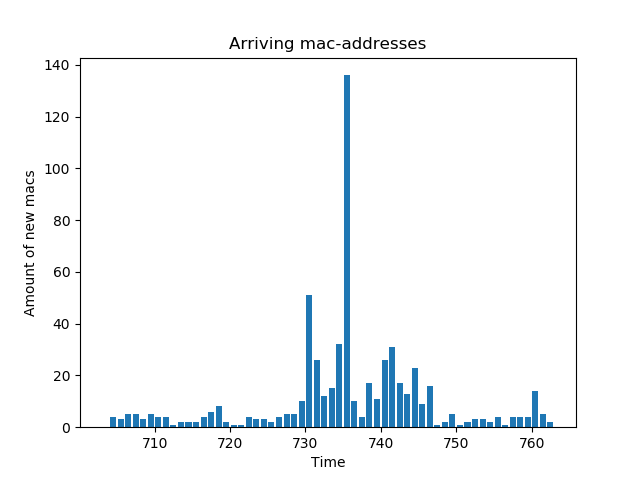
\includegraphics [width = 9cm]{images/fridaymorning7-8v2.png}
\caption{Number of MACs per time interval.\label{fig:macarrive}}
\end{wrapfigure}



Figure \ref{fig:macarrive} shows at what time how many MAC addresses arrived at the school. It is well visible that at 7:35, many students arrived at school. These students arrived with two different trains at about the same time. A few minutes earlier and after this big spike, there are a few isolated peaks. These are other trains or buses arriving. Everyone not using public transport looks like noise.

Another interesting fact that is simple to find out is if someone is a smoker or not. Because at school there is only one place allowed to smoke, I assume the people who spend above average time there are smokers or at least an excellent friends of smokers. There are still many people who walk by this stop during most breaks; that is why it is essential to also look at where they come from and where they are headed, including the time for this path and how long they stay at the smokers place.

With this data, I can retrace every step of each student and teacher. For example, it is possible to find places that people periodically visit, like their locker. Not only can I find out regularities in arrival and leaving time, but also information about their speed and direction. This means if you regularly meet your secret girlfriend, turn off your Wi-Fi; otherwise, I will see it.



\subsubsection{My Own Data}

Although my collected data has many gaps, which the data from Eduroam data can fill, my data set has one significant advantage: I could find all the Wi-Fi-active devices around, not only the ones connected to the Eduroam network, e.g., those connected to the public network. With this extra data,  I collected missing information from other Wi-Fi networks about the different devices, even if they were not as precise as the results with the Eduroam data. I found in total over 60,000 MAC-addresses (most of them only appeared once) with a total of 18'000'000 data-points per week for about six weeks. In the end, I got about 60 GB worth of metadata.

\begin{wrapfigure}[12]{c}{9cm}
\centering
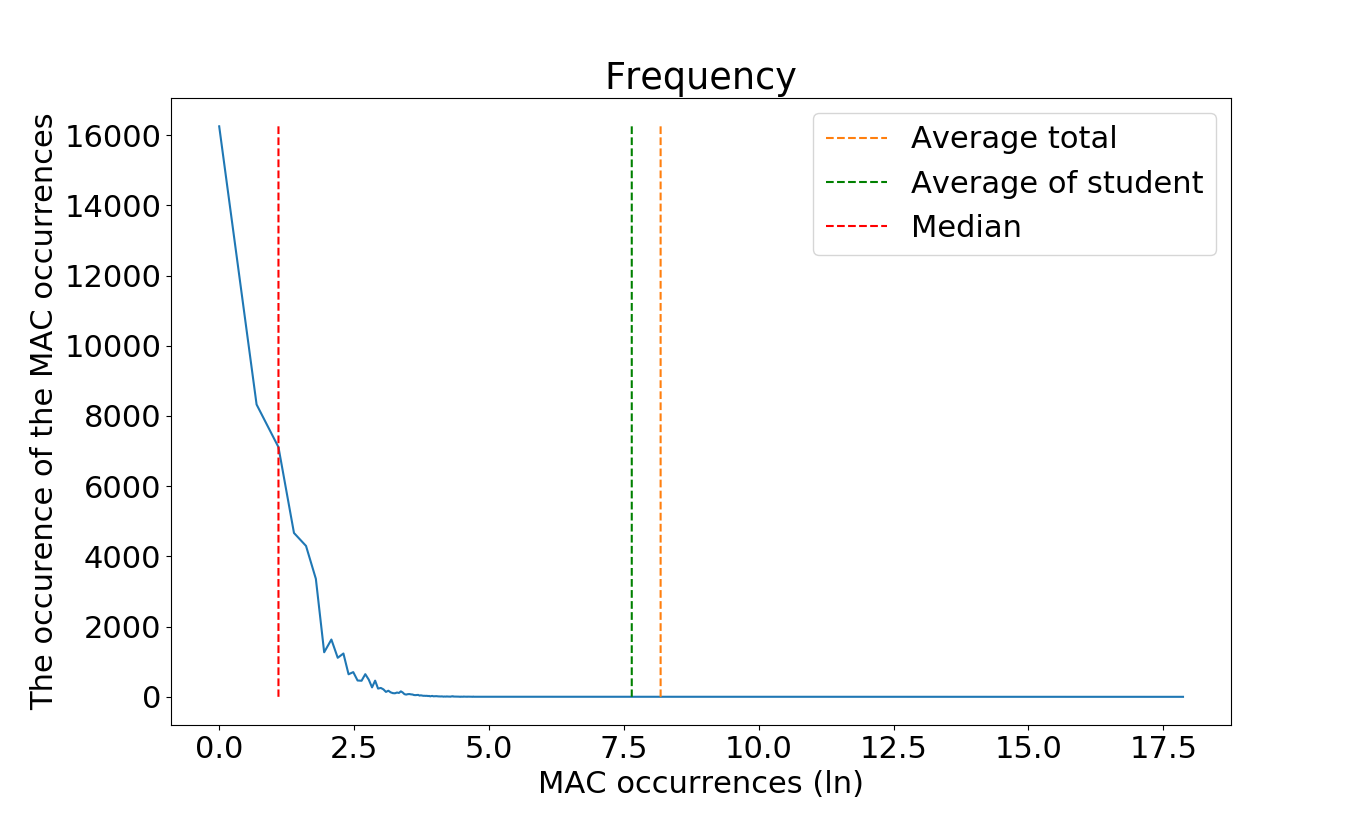
\includegraphics [width = 10cm, height = 6cm]{images/maccounter4.png}
\caption{Distribution of MAC addresses \label{usernames}}
\end{wrapfigure}

For an median student who used the demo, I got 2,094 data points, which is a little lower than the total average of 3,575. Surprisingly the median was only 3 data points! There are a lot of MAC addresses which only occurred once and there are a few with over 100,000 thousand  that is why the mean and average have a huge gape between them. The unique MAC addresses are because Apple, for example, implemented a function to use a random MAC address during the scan for known Wi-Fi networks.\footcite{applerandom}
The MAC, with the most reasonable data points, had over one million data points and belonged to an Apple device.



\subsection{Poster and Website}
\begin{wrapfigure}{r}{7.5cm}
\centering
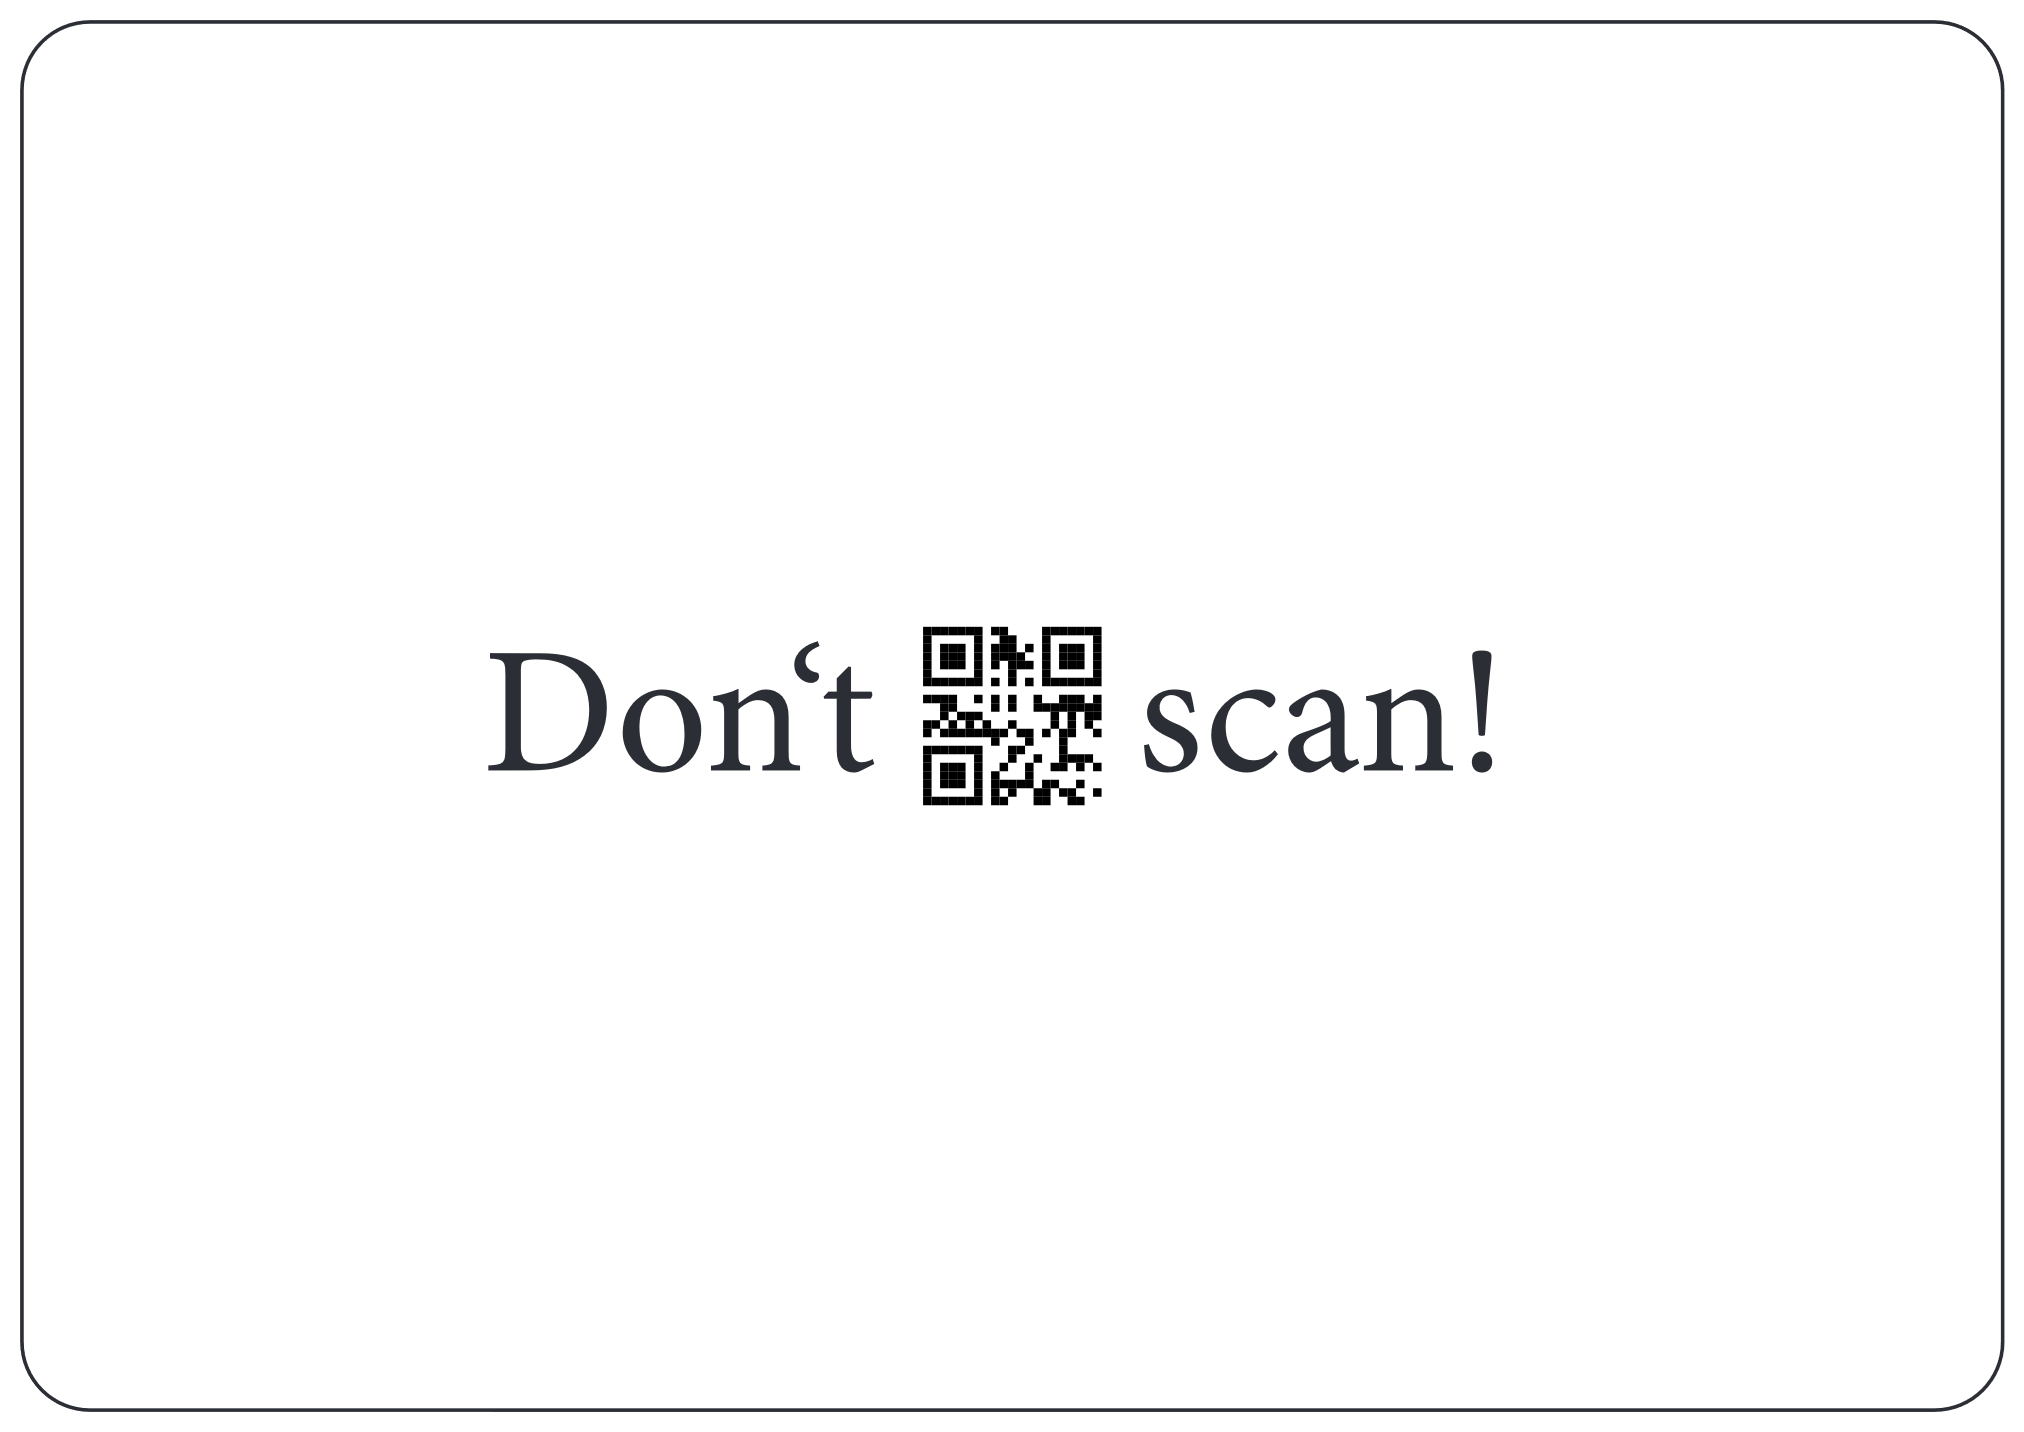
\includegraphics [width = 7cm]{images/posternice.png}
\caption{Poster\label{poster}}
\end{wrapfigure}
For spreading the knowledge about Big Data I created a little psycho-experiment. I designed posters like in figure \ref{poster} to lure students and teachers into scanning it.
The four "Don't scan" posters were hung up all around school. They were placed in the main entrance by the mensa (part of building six), in the hall towards building five and in building three (location plan in the appendix). In the first twenty-four hours, 184 students or teachers scanned the poster, and fifty-eight tried the demo. In the demo every student could find out what information I found out about them. Over the total period of two school weeks in which the signs were up, 384 curious people scanned the advertisements. Unique scans were identified by an automatic forwarding of the website. The posters were scanned most of the time during the breaks. But the demos were made mostly during a free lesson like lunch or after school. Therefore when people have little time, they may scan the posters but rarely do the demo, but with more time on their hand, they look at the website in more detail and even try the demo. Most of the students scan the poster in the mensa, followed by the one at the main entrance. This was to be expected because there are both places one waits and usually has time.




Although the posters state not to scan the QR code, many students scanned the signs because of that. This made me realize how simple manipulation nowadays could be.

For me, the success was that people were interested enough in the project to tell their friends about the posters and sometimes even helped them scan the advertisements and use the demo. Someone made their QR codes and hung them up over my posters. All of the QR lead to a YouTube video or channel. I do not know their motivation, but somehow it proves that it got noticed.

\begin{wrapfigure}[16]{r}{14cm}
\centering
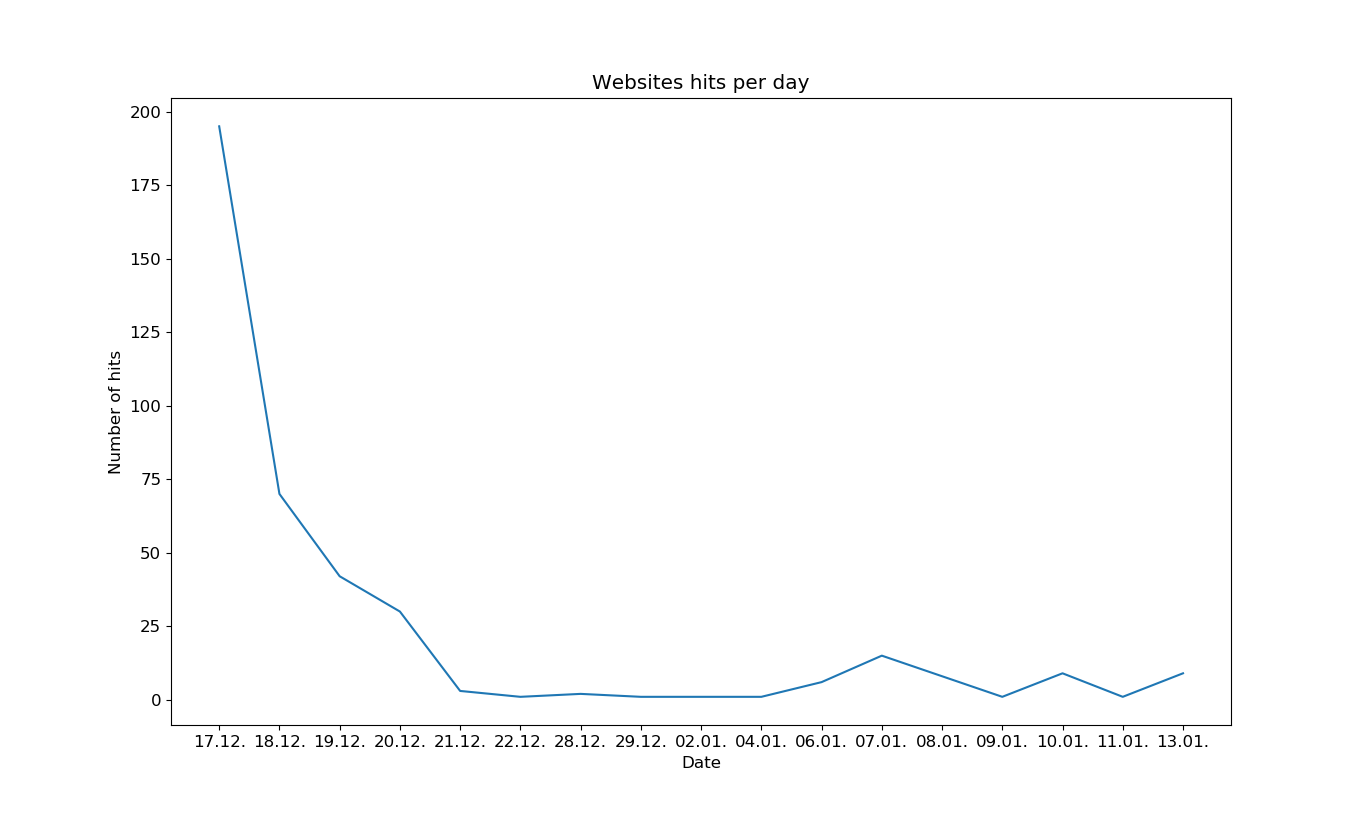
\includegraphics [width = 14cm]{images/websitevisiting.png}
\caption{The amount of people visiting my website.\label{fig:visiting}}
\end{wrapfigure}

On my website, there is also the option to subscribe to the newsletter. I only used this email once to inform everyone about my presentation. Without stating how this email was used, I still got some email addresses that scared me.

On the website, there was a sub-page that recommends a few sites and plugins to improve privacy on the web. Only 46 people used this page, but I hope I informed a few of them.

\subsection{Public School Data}
On the school website, there is more public information, which was interesting to add. With this information, I was able to match the MAC addresses to the names and precise living places. I found 95\% of all names of the Eduroam users, which is over 600 students and 120 teachers. I could not find all of them, because some used a friends credentials, or used a saved precaution to avoid being tracked (explained in section \ref{selfdefense}). I found out what the teachers studied and what they teach. I could figure out their subjects with my data. However, because the schools publish this information, it was preciser and easier to extract it from the school page. This information is published every year in a report about the last school year. Therefore these data are not the latest ones, but they change only in rare circumstances. Matching on teachers would probably be easier than compared to students, because their schedules vary wider, but this was not part of my project. Since I have access to the yearly reports of the last few years, it is possible to track the movements of teachers or students. I found out which student had repeated, switched classes, went on an exchange year, or had dropped out. With other files from the yearly report, I could figure out the number of students and use the statistics for more precise models within my data and big data.



\section{The danger behind Big Data}
Other people know my data. Many ask themselves why they should care if other people or companies have their data or not. They do not have to hide anything.
The worst thing that happens to you with public data is not that you get some personalized advertisement on your Facebook page. The danger goes far beyond that. Imagine you want to buy a house, and you need a credit from a bank.\footcite{bankscheck} The bank of your choosing runs a background check on you to be sure you are in the right financial situation and evaluates risks. These financial institutions use an algorithm with the public data and metadata from you, maybe passively, created. This algorithm tells them to a certainty of 95\% if you are creditworthy. What this algorithm searches for, no one knows precisely, and the people use it blindly. What happens to the 5\%, which are misjudged? What happens if you are among this 5\% and do not get a loan because of the model. Your life takes a big step back either by not getting a loan or by having to pay higher interest rates, both suck. This model reinforces the result by using the data generated by itself. For the bank, this is not a problem. They have trained their model to have the least amount of false positives. In other words, the bank does not want anyone not worthy of a credit to receive one. By minimizing the false positives, the false-negative usually increase. The bank does not care about a few potential customers to lose; they try to avoid risks. It is not worth to risk your career or the bank's reputation for one customer, and it is much work to do background checks by hand. But the individual, the customer is in much trouble.

The same procedure applies to any job. Before you get an interview, the company checks your online data\footcite{background}. It evaluates you without you having the chance to explain or correcting this subjective opinion. In the end, you do not even know why they did not invite you to an interview. Your future can be ruined with something that you have no control over and probably is even wrong.

The data is a subjective image of yourself, which you have close to no control over. Some people trust this information without knowing the story behind it. We tend to consider this mysterious data as evidence for this information. This means that with the data I collected, I could read anything into them. I could show specific data and claim that I have proof that a student has been cheating on a test. This is very misleading information, which often is not a hundred percent correct and can lead to wrong results. For each Big Data project, you make some assumptions, but you pretend as they were facts. For example, with my friend-finding algorithm, I assumed that friends walk together. This hypothesis is not considered when looking at the result. With losing these assumptions and forgetting the inaccuracy, this verdict has more meaning than it is supposed to have. In Big Data, the only conclusion is how well do you fit into the model provided. This model may say it can identify criminals. Still, in truth, there are just some characteristics that may or may not have a connection to crime. These models are biased in some way or another. They produce a subjective view and result in objective data.

%Nerd vs. drug addict.
I did not publish my data about smokers because it could have significant consequences for individuals. The same applies to being a drug user or a nerd. With public statistics, my data can pinpoint students within these categories. There is much information that could harm people's life. They start judging, maybe only unconscious, but the rumors getting spread and changing someone's mind is afterward a lot harder.

This is not the only way how Big Data and data collection can affect your life. Some schools use very similar systems to my project to oversee their students, and the system automatically registers the absence. .\footcite{collegestracking}
 If someone is too late, they know about it. They even can figure out if someone was late because of a late train or just makes up an excuse. These systems at those colleges use mainly Bluetooth instead of Wi-Fi but with the same idea behind it. If a student changes his phone, leaves it at home, or turns off Bluetooth, he is marked absent. The worst part is that all this happened without the knowledge of the students.\footcite{collegestracking} A poor attendance can ruin your college career without you even knowing it. In case you are on the edge of failing, the school looks at the attendance from the model and evaluate than if you stay or leave. A few people on social media suggested that students should hack these systems to show the colleges that this behavior is unacceptable. Those attacks would be illegal in the USA, and only very few students are willing to risk their school career to get freedom back. \footcite{studentrespondonsurveillance}

Very similar data collection methods can be used to find out the availability of rooms, how busy the mensa is and if the library has enough space for you to study in. \footcite{waitz} \footcite{trackingpublic} These products of Big Data are useful. They make everyday life easier, but the very same data can be used for the tracking of attendance. There is only a thin line between being dangerous or violate our privacy, and it can assist in essential aspects of life.

In general Big Data can gather much information of harmless metadata. This data can be used in many different situations, but all of them carry a particular risk with them. In some cases, these risks are that you get the wrong targeted advertisement on your Facebook page; others can ruin your life or cost you thousands of francs.

\section{Are tracking methods legal?}
During my project, I looked at the Swiss Data Protection Law and realized that I am moving in a gray area. I am allowed to collect the depersonalized data. Splitting the data into groups is permitted as long as the groups contain more than one person.\footcite{swissdataprotection} This is the case for my work because every class had at least fifteen students and the place of residence was not precise enough. The rest I found out only from assuming and cannot be completely validated.

The problem was combining my data and the information I found online. The information I found online was very personalized, and with trickery, I could add them to my dataset.

The data I collected and the information I gather out of my data were utterly legal and depersonalized. Merging this information with the info, I found online is in a gray area.

Since I used my project to inform the school about the danger of Big Data and rise awareness, I can argue that my action was in the public's interest in improving and expanding their knowledge. The law states that it is legal to track humans in public spaces if the public benefits from it. This law is usually used for traffic control and human flow. \footcite{swissdataprotection}

Further, I split my results, in this paper and on the website, into two sets. The first set that I got from my data and its analysis is entirely legal. The other set is just a collection of data the school publishes. The second set of results is as legitimate as looking up the capital of Norway.

For more detailed, personalized, and win oriented profiles, the Swiss Data Protection Law requires the consent of the targeted person. Getting these permissions can be hard for projects like mine. Still, companies with websites or a product to sell, have stated it mostly in their business conditions. "By using our product, you give us the right to collect personal data on you."
With these cookies or conditions, companies get your permission to collect data on you. These companies are not allowed to give the data to third parties (Art. 12 DSG)\footcite{swissdataprotection}. There was an incident when Google, on its camera tours, collected Wi-Fi data. This event happened in 2010, and the Swiss government was shocked by how much-unencrypted data Google could collect. For this violation, the Swiss government forced Google to pay fines and made them to delete all the collected data. \footcite{googleadmin}


Lately, in the news, there were discussions about the new data protection laws in the European Union. These laws were made to give basic rights of data privacy to every citizen. They should protect the private data of each person. These laws state some important and necessary rules to follow when doing data capturing, analysis, and information gathering. \footcite{dsgvo}
It includes that it is not allowed to capture data that contain strictly private information like race, political opinion, religious believes, and biometric data. Like too many other laws, this one has ten special cases where this rule does not apply. One of these exceptions backs my project up. In subsection (2 a), it states that information can be used if the person already has the data published like the school has published the place of residence for each student. \footcite{dsgvoart9}
This makes my combination completely legal.

These data protection laws are more advanced and modern than the Swiss laws, which is why we probably will sooner or later adapt to them. These laws give a basic guidance for what data can be collected and stored. Some consider this step as a block of our future, but I believe these laws give us, at least in theory, some control over our data back.

When we look towards the United States, often considered more advanced in the technological field, we discover they do not know what data protection even means.\footcite{usdataprotection} They look at data protection more as an obstacle than a fundamental human right.
The laws in the United States are a lot liberal and less supervised. With the new rules in the EU, that many US companies have to follow, the USA gets under pressure. But at the moment, if you want to send a package from the US post office and pay with your credit card, the return address is filled out for you. The bank sends your home address to the postal service. For us, that is a massive violation of privacy. In the USA, banks sell it as a feature.

In the United States of America, people have different values. They are willing to give up their privacy for comfort and simplicity. In the process of giving up one's privacy, many things get more comfortable, like meeting friends. When you always share your location with anyone, you know when friends are close to you, and you can hang out. Amazon, for instance, may find a way to send you packages without you requesting it. The crime rate could decrease if everything were public. But with the release of all data, also problems arise for example that companies and governments are obligated to publish their secrets that could lead to the death of capitalism. The companies lose their economic advantages because everyone would know the secret recipe. Nowadays, this counts as insider trading. If we would allow these organizations keep secrets, why not humans. Our secrets can be as important as one's companies. There are a lot of other questions which lead to further problems.
Comfort sounds nice to have, but in the end, there has to be a solution in the middle between privacy and publishing data.

The cloud, the newest and most popular service in the internet nowadays, is most of the time offered by a US companies. Therefore US laws apply. We know that these companies have the option to read our data! They promise not to look at our files. However, it is impossible to control violations not only with clouds but with all the digital data. The companies are not willing, out of different reasons, to publish their Big Data tools.

\section{What else can track me?}
Monitoring people with Wi-Fi metadata and their MAC-addresses is one method. However, there are several other methods, which are sometimes more fitting for the purpose, like for example, Radio-Frequency Identification (RFID)\footcite{studenttracking}. RFID is a communication format often used in security batches, library systems, and in many cards\footcite{datenschutzrfid}. The SBB "Swiss Pass" also uses this technology to get information about the owner. Every time you show them your card, they scan it and save the information that you were on this train \footcite{sbbdatenschutz}. Soon, I believe, we have to carry our card and walk into any train we want, and SBB books a ticket for us automatically, for the lowest possible price. This little feature provides them with people's location every time they use their services. Knowing exactly which tram one take and who else is there, they can find out an enormous amount of information about nearly every Swiss citizen. Officially these features are used most of the time for analysis how the different train or tram lines are occupied with, allowing them to optimize the connections and avoiding delays.\footcite{miningtransport}

The Swiss Pass is not the only card in your wallet, that gives others the ability to track you. Your credit card has the same option. Most new debit or credit cards have the features to pay contactless. This innovation helps stores to be able to track you through the whole store, including what you buy (mentioned in the introduction). The contactless credit card chip only works for a few centimeters. Still, some experiments showed it works perfectly up to 0.9 meters. \footcite{contactlesspaymentsppp}This is the perfect distance for stores. With further distance, the data loss is too much, and the cards cannot be distinguished.
\footcite{contactlesspaymentspaper} 

Besides cards, there are many devices or features, that let you be tracked. Nearly every device which transmits any information over air makes you trackable. That also includes common by Bluetooth devices like wireless headphones or digital watches. They have a constant connection to one's phone, and with a range of about 10 m, it is very similar to Wi-Fi. The encryption is also very similar to Wi-Fi, and Bluetooth also uses something like a MAC address, but the pairing is entirely different. If someone listens to the pairing of the Bluetooth device, it is possible to break the encryption and listen to the music played on the headphones or the phone call made with the headset. \footcite{ubertooth}

There is a tool, similar to the WiFi Pineapple, for Bluetooth sniffing, it is called Ubertooth. \footcite{ubertooth} I had the option to use this tool, and when applied correctly, it has many choices. I could have used Bluetooth, but the downside with Bluetooth is that it is only active when used. If you are listening to music on your Bluetooth headphones or are connected with your digital watch, it works as well as Wi-Fi. Still, a typical user uses more often Wi-Fi then Bluetooth, and Wi-Fi sends information in the background to search for networks, updates, or stream music or a video.

Although it is not as easy to process, video surveillance is also an excellent way to track objects or people. This method can gain you much more information like color or size, which is harder to determine with Wi-Fi signals.

A method which is often forgotten, but helps for surprisingly many to track are social media websites. This website can track your approximate location and your time and amount of usage. This information can be useful for Big Data, but there are more information in the public posts of the users.Many, especially Swiss people, have a certain awareness of the risks involved by posting their location and the story of their life on these platforms.

Nowadays, with modern technologies, it is hard not to be tracked. There are dozens of options on how to trace someone. Nevertheless, we cannot forget that this is not the intentional way of using this technology. Similar to a bread knife not being a killing tool. We need to know who we trust with this information and realize when we give them the possibility to track us and when we keep our personal information private.

These are all passive attacks. Passive means that I am just collecting data sent by devices anyway and not forcing them to create any. As soon as the attack gets active, it often goes under hacking. This includes viruses, malware, ransomware, but also simple pinging ones phone. These attacks are even harder to protect from, but usually, they happen less on a big scale and in the background. That is why I do not focus on them during my paper.



\section{Defense}
\subsection{Self Defense}
\label{selfdefense}

Completely protecting yourself from Big Data is a nearly impossible task nowadays. Unless you are ready to abandon your home and life on a remote island without any electronic devices, Big Data manipulates you and has some control over you. But understanding how it works enables you to have as much power as possible. All this without losing too much comfort.

First, let us look at my big data project. With a mobile data plan and deactivating your Wi-Fi, I cannot detect you anymore. This raises the bar; the equipment to listen to the mobile network is much more difficult to access. But in this case, you give the possibility to trace you to someone else, e.g., Swisscom\footcite{swisscomads}.
It becomes harder when you try to hide from Swisscom or other companies. Most of us are depending on them in one way or another. There are still some tricks to make it more difficult for companies to trace you. Against common believes using a VPN does not help to hide the websites you are browsing. It only protects you from your curious internet provider, but the company operating the VPN gets all the information.\footcite{tomscottvpn} This is similar to avoid my tracking attempt but giving Swisscom all the info.

You can limit real-world tracing by putting your phone into airplane mode when you do not need to be reachable or browse the Internet or use Bluetooth. For credit cards, there are cases or wallets which block the scanning of these devices. To avoid online tracking, there are many websites like duckduckgo.com that promise not to track you. It is very much recommended to refuse giving personal information like phone numbers and email addresses, if possible.

Completely stopping wireless tracking is possible with a Faraday cage. This is a box where no electromagnetic signals can pass through. The metal reflects the waves from all sides of the cage. In this cage, one is not traceable from the outside through these waves, but there is also no Wi-Fi nor Bluetooth signal from the outside. It is like a little island without connections to the outer world. There are also phone bags that are not letting a message through. These could make a lovely purse, maybe, but otherwise not very user-friendly nor popular.

A more user-friendly option is to turn on MAC randomization. This changes your MAC address every time you connect to a Wi-Fi, which makes it harder to impossible to track. Android, Windows, and Linux officially support MAC randomization. \footcite{randomwindows}\footcite{randomandroid} \footcite{randomlinux} There are certain Wi-Fi cards that do not support the randomization. \footcite{randomwin10} Sadly, it is not supported on Apple devices and, as said, not the standard on any platforms. It is possible with macOS, but not with the builtin tools. \footcite{randomapple} The MAC randomization would render my data useless. There is a downside to the security. No public Wi-Fi will remember you, and you have to pass the registration procedure every time you reconnect.

Furthermore, the randomization built in to any phones or laptops is not secure. I found a paper that shows a method of how to unscramble the MAC and find the real MAC address. \footcite{notrandom}
This is due to an implementation failure on all platforms, which provides the real MAC address if asked correctly. Therefore it is impossible to use the Wi-Fi and completely hide one's identity. Still, you can make it very hard for the tracker.

The random address is useless when the username stays the same. Then instead of tracking the MAC, I look for the usernames. This can be prevented by changing the protocol from EAP-PWD to Protected Extensible Authentication Protocol (PEAP). EAP-PWD sends the real username unencrypted in the metadata, PEAP does not  when configured to use an anonymous outer identity. With this, it is possible to change the unencrypted username to an anonymous one. I recommend either "anonymous" or "eduroam" to have a minimum matching. With the combination of random MACs and a hidden username, there is not much I can track.


At the moment, there are about a handful of teachers or students that use PEAP correctly, and only one of them uses random MAC scrambling out of the about 2000 users. This means I can identify all of them either by the MAC or by the username. This should show that if only a few use these strategies, it does not make it more secure. It even can have the opposite effect. But as soon as you convince enough people to change to the more reliable way, the work for tracking individuals increases enormously. Imagine that you start dressing in a full diving suit. If everyone would wear this way, it is tough to track anyone. But if you are the only one doing this, you stick out way more than before. Quite ironic! This is the same with some protections against Big Data.

A good rule is only to use and produce data if necessary, and change usernames, passwords, and MAC addresses regularly.


\subsection{What the school can do}

\subsubsection{Wi-Fi}


First and most importantly is that the school should use anonymous usernames for the Wi-Fi. If the first and last name is in the username, the information gathering becomes a lot easier. I identified 60\% of the users only with their usernames.



To avoid this tracking, the school can use six random letters. The usernames would look like ragoqx@edu-zg.ch instead of lohr.nico.2013@ksz.edu-zg.ch. I would also remove the "ksz" from the username to decrease the information hidden in this name. There are over a billion combinations, so there should be enough for a long time. Each user can use a different username for each device. It is also recommended to change the username frequently. If every student requests ten new usernames a day, this could go on for more then thirty years.

Using CAT protects you even better.\footcite{cateduroam}
This configures the phone automatically to use the most secure protocols and hides the username. Without usernames at all, I have to rely on the MAC addresses to identify the different devices.

\begin{wrapfigure}[13]{c}{11cm}
\centering
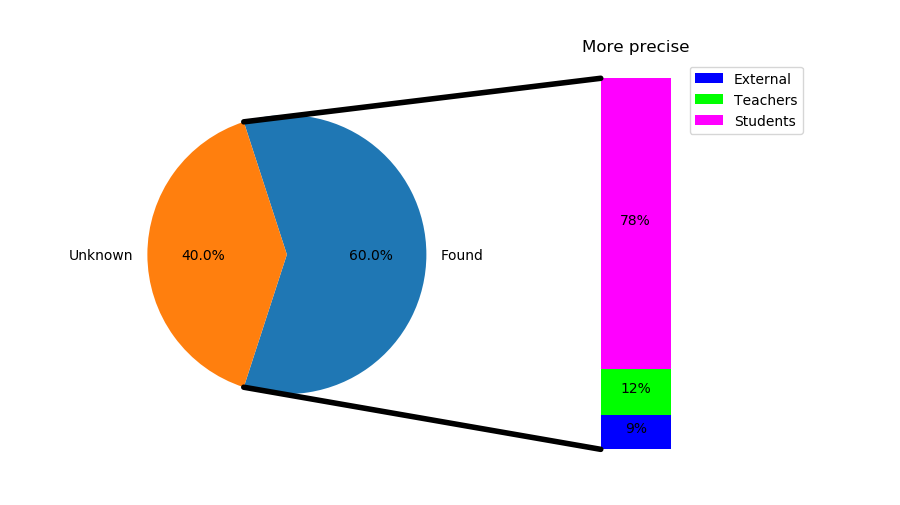
\includegraphics [width = 12cm]{images/piecharwith_usernames.png}
\caption{Usernames found \label{usernames}}
\end{wrapfigure}

Although our public Wi-Fi does not use a username that allows being identified, public Wi-Fi has a much bigger problem. The data transported between the access-point and the phone is not encrypted at all. This gives everyone around the possibility to check on what website you are. To increase privacy, one should turn off public Wi-Fis. This has some disadvantages and causes other problems. For example, one needs Wi-Fi to connect to the Eduroam network. A realistic approach is to make the public Wi-Fi annoying to use, force the user to login every day or even like the SBB-Free Wi-Fi every hour.



An option to consider, but most likely not possible with the current infrastructure, is an LTE campus network.
Such a campus network works similar to Wi-Fi, but it uses better encryption and different frequency, which makes it a lot harder to collect.

\subsubsection{Reduce the digital footprint}

The school made it very easy for me by publishing every student's full name and place of residence on their website. This is not acceptable! All these data that have private information in them should only be accessible after a secure login, with a password or only internally form school. This not only counts for names and places but also for time tables. Every information published on the website, especially collected information like a datasheet, helps to improve and expand profiles of everyone involved. The yearly report should be anonymous if publicly available.

\section{Further Ideas}
An old idea I had, which would go into a little bit of another direction, would be building my own WiFi Pineapple. I would focus on making the devices, I thought of an Arduino, so small that I could place it in a power plug. This makes it perfectly invisible, it has enough power, and it can be placed at many different places. The problem so far with this idea was that there is no good library that enables monitoring mode on such small devices. These devices would have given me the possibility to collect all the produced metadata. Because these little Arduinos costs nearly nothing, I actually could afford it.

An active attack I had in mind would be throwing everyone off the public Wi-Fi at school and letting them connect to my hotspot. With this method, I could get the mobile number of these students. This would violate too many laws so that I did not do it in the end, but the plan exists. With rerouting all the traffic over my device, I also could access the website they are searching for or their Instagram login.


There was a university which used something similar to my early idea to monitor how busy the library, the lunchroom or the kitchen was in real-time.\footcite{waitz}
Finding regularities in data and the behavior of students could lead to interesting results. \footcite{deanonymisationmac}
This idea does not use big data and is more focused on data collection, but it can be helpful to know when the right time is to eat lunch. So far, we have to rely on our guts.

With more data, I thought it would be hilarious to create some statistics about our school. Like how often does an average student go to the restroom, or how many people are ill each day? Maybe there is a difference between November and December with the number of sick people. This could help detect biases in the Big Data system but is not Big Data itself.


Knowing every student's move is fun to know, but it is hard to read out of these files. I thought about making a 3D model where I visualize the movement of every student and teacher at school in the hallways (and rooms). This could not only look fun but also could help finding the least busiest path from A to B.

The first proof of concept was to differentiate classes. Still, I was wondering if an algorithm also can figure out the difference between the WMS and the Kanti students or the students and the teachers. Generally, what other groups can be found in this pile of data. I hoped to find these groups with a few advanced algorithms, but with too many random data, the algorithms failed. I still want to try this again.



An idea I got lately was that I could connect my result to a targeted google search or the online phone book to find more personal information like the address. I know with the school name, my name, and my place of residence, it is possible to find a few more details about me online. This again has some potential legal problems, but I thought it would be nice if I greeted the user with an image of them (google search) when they enter their MAC-address on my website.



\section{Limitation}
Big Data can find out much information about a person, but there are still some limitations. Like in my project, the lack of data can be a problem. If you do not have enough representing data, you cannot produce the result with the accuracy you need. This is already the second problem. Most of the time, Big Data is used to generalize things, and there is always an exception the model is not covering. The accuracy has limitations and is hard to measure, especially with an unspecific number of users. Having the wrong data is also possible. I could never find out what you were talking about with your friends by the Wi-Fi metadata only. With cameras and lip reading or just audio, this can be done a lot better. This would be more spying the Big Data, but can also be used for Big Data related projects. In my project, on the one hand, the repetition was interesting, the time-table and the habits, but on the other hand, the data-points which stuck out of order. These could tell me if someone missed school, but Big Data (with only my data) would never find the reason why this student missed. With my data, I could figure out a lot on campus, but as soon as it was off-campus, it got unprecise and random. Of course, this would change if I got more data, for example, from the Metalli or Swisscom.

\section{What have I learned the hard way}
Time management would have been vital! Everything took way longer then I expected. Big Data works best when you have "big" amounts of data. I underestimated how much data I need to get decent results. Besides the collection of several week's worth of data, I needed to parse all the data I got. This process took half a week again, and the loading times from the further proceedings with my data were not much faster. Small errors in the work with these amounts of data can be a setback for several days. It is essential to test the code first with a little simulated scenario before waiting hours for the wrong results.

Contrary to my beliefs at the beginning, I was not able to create all my results with simple python programs and the counting method. The more data and more complicated goals I had, python was to slow, and the counting method got too complicated, I had to switch to more advanced algorithms.

Besides some software and programming problems, I also had some hardware problems. The WiFi Pineapple was plugged out of the power plug several times in different ways. One time the cable reel was suddenly gone and never seen again.

All of these problems were factors that, in the end, I did not have as much data as I hoped and cost me much time.

I had to deal with time zones and different settings of time, which made the whole process harder. My computer, the WiFi Pineapple, and my data all had different time zones or time formats, which made it hard to match to the correct time. If the times in the data are off by a few minutes, the entire algorithms return the wrong results.

Problems with my website were surprisingly small. I was lucky that the process never crashed when the posters were up. In testing, I locked my self out of the server a few times.

I misjudged the time needed to hang the posters. I did not release that the process had so many steps. First, one needs to design the banners, then print them, and just then, I could ask for permission to hang them. Fortunately, they allowed the posters.


\section{Conclusion}
For a Big Data project, one needs big data, but we produce enough every day for thousands of projects. My results were not perfect by a long shot. Still, I could find out much information about students as well as teachers. This was done only by a few weeks of punctual data collection. With the posters and the website, I could shine a new light on the topic and, with my approach, made it enough personalized that people started asking questions. This is a crucial part of Big Data. You cannot completely hide from Big Data, nor do anyone want to. These algorithms have positive aspects, and we are not allowed to forget that. Still, knowing how they work, we can protect ourselves from the negative side. This includes not only the Wi-Fi-metadata but also all other possible tracking and data-producing technologies. My manipulation on the poster showed that simple reverse psychology works very well today. With the over 300 hits on the website, I hope I helped a few get a new grasp on Big Data and its vast potential. Which contains big risks and dangers; that is why it has to be regulated.
In Switzerland, we have the luck that the laws prohibit a lot of Big Data methods that attack our privacy. This ideology that privacy is something to protect is spreading through international laws slowly, even to the United States. Still, we accept conditions that attempt to kill our privacy nearly every time we go on a website.

Big Data is not hard to create, but it can be powerful. If you know the daily usage and the possibility of manipulation, it helps to spot, question, and avoid these situations. With a little bit of care and extra work, it is possible to make the profiling for big companies a lot harder.

It was possible to find out a scary amount of exciting information with no experience, limited resources, a small budget, only passive listening, and all that legally.
That makes me wonder: What do the big influential companies and government know?


\section{Thanks}

I wish to thank my school for providing the infrastructure I could use for my project, Marco Schmid, for the support and guidance during the project, Christian Wittenhorst for helping me with the school infrastructure, providing the data and answering technical problems and Hansjörg Grünig for correcting and improving my English.

\section{Bibliography}
\printbibliography


\listoffigures
\end{document}